\documentclass[11pt,a4paper]{article}
\usepackage{ls}

\usetikzlibrary{shapes}
\usepackage{xcolor}

\usepackage[english]{babel}
\setlist{noitemsep}


\newcommand{\HGG}[1]{\begin{quote}\textbf{Anmerkung HGG:} #1\end{quote}}
\newcommand{\todo}{{\color{red}\textbf{ToDo}}}

\newenvironment{code}{\tt \begin{tabbing}
\hskip12pt\=\hskip12pt\=\hskip12pt\=\hskip12pt\=\hskip5cm\=\hskip5cm\=\kill}
{\end{tabbing}}
\def\dq{{\char34}}

\title{A Proposal for Modelling TRIZ Functional Analysis}

\author{Tarek Stelzle}

\date{Version of April 11, 2021, revised version of July 9}

\begin{document}
\maketitle
\tableofcontents
\clearpage

\section{Aim of the work}

The aim of this paper is to elaborate a proposal for an ontological modelling
of the area of \emph{TRIZ Functional Analysis} based on the approaches in
\cite{KS}, \cite{WebinarFunctionAnalysis}, \cite{SouchkovGlossary} and further
own investigations.

The work fits into the activities of the \emph{WUMM Ontology Project}
\cite{WUMM} to model core TRIZ concepts using modern Semantic Web means.  The
work consists of two parts -- a \emph{Turtle file}, in which the semantic
modelling is performed based on the SKOS framework \cite{SKOS}, and \emph{this
  description}, in which the background and motivation of the concrete
modelling decisions are detailed.

The paper is structured in the following way.  In section 2 the information
sources are mentioned and further discussed.  In section 3 we shortly explain
the conceptualisation.  In section 4 the Functional Analysis as described in
\cite{KS} is summarized.  Section 5 introduces Python tools which have been
implemented to make the \emph{Turtle} file easier to create.  In section 6 it
is shown how and why the \emph{Turtle} file has been created in that way.
Section 7 contains some example implementations of the \emph{Turtle} file for
Functional Analysis.  In section 8 some conclusion are given.

\section{Starting point} 
\label{sec:starting_point}

The starting point for building the ontology for Functional Analysis are the
explanations in \cite{KS}.  The definitions, demonstrations and explanations
given there are used within the implementation of the ontology.

Other notations and definitions from Functional Analyis are taken from Valeri
Souchkov's Glossary \cite{SouchkovGlossary} as a comprehensive source of
well-established definitions.

These two information sources and the material from Nikolai Shchedrin's
webinar \cite{WebinarFunctionAnalysis} are the main sources used to build a
proposal for an RDF-based TRIZ ontology for Functional Analysis.

In that webinar Nikolai Shchedrin developed the modelling basics of an
ontology for \emph{Functions} and \emph{Function Analysis} and presented some
considerations on how to structure this part of the TRIZ ontology.

\subsection{Classification of Functions}

First he proposed to divide the functions into three types:
\begin{enumerate}
\item Functions of the subsystem,
\item Functions of the supersystem,
\item Functions of the surrounding objects.
\end{enumerate}

\subsection{Model of a Function and the Functional Model}

Furthermore he introduced the \emph{Model of a function}.  This model
describes the properties of a function is. This covers not only the action and
the two components which interact, but furthermore the parameters, the type of
the function and the degree of execution.

The \emph{Functional Model} is a graph representation of the system to be
analyzed.  Every node in the graph is a component or a subsystem of the
system.  The functions are represented by edges.  This is further explained in
\ref{subsec:functional_model}.

The \emph{Model of a function} can be helpful for building the
\emph{Functional Model}.

\subsubsection{Objectives Of A System}
\label{subsubsec:objectives_system}

As explained by Nikolai Shchedrin the objective of a system can be divided
into three objectives.
\begin{enumerate}
\item Primary Objective
\item Secondary Objective
\item Auxiliary Objective
\end{enumerate}

The \emph{Primary Objective} is the objective, which the system was build for.

\emph{Secondary Objectives} of the system are functionalities which are
offered by the system, but for which it was not mainly built.

\emph{Auxiliary Objectives} fulfill the purpose to get the Primary Objective
to work.

\subsubsection{Primary Function}
\label{subsubsec:primary_function}

Furthermore a function can be classified in one of these three functions.
\begin{enumerate}
\item Primary Function
\item Core Functions
\item Auxiliary Functions
\end{enumerate}

The \emph{Primary Function} serves the Primary Objective and its technical
execution.

\emph{Core Functions} represent functions, which directly support the Primary
Function.

\emph{Auxiliary Functions} describe the set of functions which help to run
other subsystems.

\section{The Conceptualisations}
\label{sec:conceptualisations}

The conceptualisations to be developed follow the basic assumptions and lines
that are elaborated in more detail in \cite{Graebe2021}. In particular, the
following namespace prefixes are used:
\begin{itemize}
\item \texttt{ex:} -- the namespace of a special system to be modelled. 
\item \texttt{tc:} -- the namespace of the TRIZ concepts (RDF subjects).
\item \texttt{od:} -- the namespace of WUMM's own concepts (RDF predicates,
  general concepts).
\end{itemize}

The concept will be to gather various definitions from the mentioned sources.
With these sources the important TRIZ triple will be implemented.

From there the necessary connection will be created for the various triples.
Furthermore missing concepts will be introduced to fully expand the modelling
of Functional Analysis and related concepts.

For the organizing of the turtle file and to structure the building process of
the turtle file, first of all the Functional Model will be built.  This is
done by following the five steps, which will be explained in
\ref{subsec:functional_model}.  With the given model the Functional Analysis
components can be added to attach all important concepts.

In the end the implementation will be supported by different example, which
are going to use the implemented concepts.  In figure
\ref{fig:example_conceptionalism} an implemented function of an example is
shown.

\begin{code}\tt
  ex:Steer\\
  \> a tc:function ;\\
  \> tc:SubjectActionObject ex:DriverTurnSteeringwheel ;\\
  \> tc:QualityOfFunction tc:UsefulFunction ;\\
  \> skos:prefLabel "Steer"@en ;\\
  \> skos:Definition "Turning the steering wheel by the\\
  \> \> driver to change the direction of the vehicle."@en .
\end{code}
%\caption{Example For Function \emph{Steer}}

\section{Functional Analysis}
\label{sec:functional_analysis}

In this section a summary about the terms and definitions explained in
\cite{KS} will be given.  This is going to help explain in the following
sections, why the \emph{turtle}-file was modeled in that way.

\subsection{Concept}

In Functional Analysis the idea is to represent a system by various functions.
This representation helps in organizing and structuring the system.  To tackle
the optimization problem a more precise look is taken at the non-useful and
contradictory functions in the system.

The two main objectives of Functional Analysis in TRIZ are formulated in the
following.
\begin{enumerate}
\item Recognition of problems.
  
  Hereby the objective is to find as many as possible non-useful or
  contradictory functions in the system.
\item Trimming of components.
  
  Redesign or remove components to optimize the system.  During this process
  the functionality of the component must not be changed.
\end{enumerate}

With these two main objectives there are five tasks to handle in Functional
Analysis.
\begin{enumerate}
\item Recognizing Interactions Between Objects
\item Recognizing Problems Within The System
\item Formulating Open Problems
\item Innovative Redesign
\item Optimizing Systems By Trimming
\item Bypassing Patents
\end{enumerate}

\subsection{Quality of a Function}

To further analyze the functions it is recommended to give each function a
level of quality.  This quality of a function makes it easier to find problems
within the system.

According to the book there are five different quality levels.

\begin{enumerate}
\item Useful function: \\  
  A function works as intended and the result is only positive.
\item Useful, but insufficient function: \\
  A function has a positive impact but the result is not satisfying.
\item Useful, but bad controllable function: \\
  A function with a positive impact but is not satisfying as the result cannot
  be controlled.  Hence it is wrongly timed.
\item Useful, but excessive function: \\
  A function with a positive impact but a heavier result than necessary.
\item Harmful function: \\
  A function which has a negative impact.
\end{enumerate}

More precise definitions can be found in the book \cite{KS} or in Souchkov's
glossary \cite{SouchkovGlossary}.  As both of these are merged into the
\emph{turtle}-file the defintions can now also be found there.

Nikolai Shchedrin mentioned also a new function quality in his web-seminar.
This is called \emph{Useful function with disadvantages}.  As mentioned on the
website \cite{ShchedrinUsefulFunctionDisadvantage} this class includes
Redundant Functions, Insufficient Functions, Bad Controllable Functions and
Missing Functions.

As there is no source mentioning the definition of a Redundant Function and a
Missing Function, these will be interpreted in the following way.
\begin{enumerate}
\item Redundant Function: \\
  A useful function, which is implemented several times in the system.
\item Missing Function: \\
  A required useful function which is not (yet) implemented in the system.
\end{enumerate}

\subsection{Functional Model}
\label{subsec:functional_model}

The Functional Model structures the function and the components in the system.
In the book the following steps are recommended when building a Functional
Model.  It is also mentioned that steps two to four can be made in one step.
\begin{enumerate}
\item Making a list of components
\item Determine interactions
\item Linking functions to components (subject)
\item Determining the direction of function (arrow)
\item Define the quality of the function
\end{enumerate}

With this a graph-like structure is built.  Every node in this graph
represents a component or subsystem within the system.  An edge represents a
function.  Different styles and forms of an edge represent the quality of the
function.

For easier reading and analyzing the Functional Model, it is possible to group
components according to self-defined properties.

\subsection{Positive And Negative Aspects}

Using Functional Analysis helps you to fully understand a system under
examination.  Furthermore you can exchange knowledge between colleagues and
fix misunderstandings.

Functional Analysis makes also sense, when no problem is known.  This is good
if you want to improve your system without knowing specific complications.

A negative attitude of Functional Analysis, is that only known systems can be
analyzed.

\section{Implementation of Tools}

\subsection{Creating Turtle File}

For easier and faster creation of the "Matrix 2003" a small Python tool was
implemented.  This tool reads the matrix from a \emph{csv}-file and generates
a \emph{turtle}-file.

\subsubsection{The CSV-File}

First of alle the \emph{csv} file needs to be in the following syntax, because
otherwise the matrix is wrongly interpreted.  Every line in the csv file is a
row in the matrix.  Furthermore every comma separates a column entry in a row.
The different entries in the matrix field are separated by dashes.

For reading the matrix the tool "tabula" was used \cite{tabula}.  With this
tool the Matrix2003 from the book "Systematische Innovation" was interpreted
as a txt file.  As this did not have the right syntax the small script, named
\texttt{convertTxtMatrixToCsv.py}, was created.  With this the matrix is
converted into the right syntax, as mentioned above.

Usage of the script: 
\begin{quote}\tt
    python convertTxtMatrixToCsv.py $<$csv-file-name$>$
\end{quote}
This creates a \emph{csv}-file \texttt{createdMatrix.csv}.  The file
\texttt{temporary.txt} is a temporary file. It can be deleted afterwards.

\subsubsection{Creating The Matrix}
\label{subsubsec:creating_matrix}

The following explains the implementation of the \texttt{createMatrix.py}
script.

The script uses three other files.  The first is the \texttt{principles.txt}.
In this file all the fourty principles are written down, with their belonging
number at the beginning.  Hence the script can map an entry index to the
belonging principle name.

The second file, which is also used is called \texttt{parameters.txt}.  In
there are all the fourty-eight parameters which represent the column and rows
in the matrix.  These names are similar to those for the Altshuller Matrix.
The nine new parameters, which were introduced for the Matrix2003 are the
following.

As this matrix introduced upper-parameters, a third file for these is needed.
This has been called \texttt{upperParameters.txt}.  The upper-parameters are
linked by writing the upper-parameter number with a dot before the parameters
in the \texttt{parameters.txt}.  The python script then handles the rest.

\begin{enumerate}
\item QuantityOfInformation
\item FunctionEfficiency
\item Noise
\item HarmfulEmissions
\item CompatitbilityOrConnectability
\item Security
\item Vulnerability
\item AestheticsOrAppearance
\item ComplexityOfControl
\end{enumerate}

The layout for the Turtle file is the same as the layout for the "Altshuller
Matrix".  As this makes it easier for later adjustments or improvements of the
matrices.

At first the script creates the header for the Matrix2003, which is the same
as in the "Altshuller Matrix".  Then it defines the owl entry for the Matrix.
Afterwards the script iterates over the entries in the \emph{csv} file and
builds the matrix in the following way.

\begin{figure}[ht]
  \centering
  \begin{code}\tt
    <http://opendiscovery.org/rdf/Matrix/E.06.34>\\
    \> od:upperDecreasingParameter tc:Non-Functionality ;\\
    \> od:decreasingParameter tc:EaseOfUse ;\\
    \> od:upperIncreasingParameter tc:Physical Parameters ;\\
    \> od:increasingParameter tc:SurfaceOfTheStationaryObject ;\\
    \> od:recommendedPrinciple tc:PreferredAction, tc:Asymmetry, \\
    \> \> \> tc:Mediator, tc:SelfService ;\\
    \> a od:MatrixEntry .
  \end{code}
  \caption{Entry of the Matrix2003 Turtle File}
\end{figure}

The script is started with the following command:
\begin{quote}\tt
    python createMatrix.py $<$csv-file-name$>$
\end{quote}
This creates a file \texttt{created\_matrix.ttl} with the result of the
transformation.

\subsection{Translating}

For translating the various tags a Python script was implemented, which takes
a turtle files as input and adds the missing language tags.  Therefore the
script checks each line which already has a language tag.  Then it makes an
api call with the first tag as the source language.  It adds the language tags
for English, German and Russian.  Each tag is a separate api call.  For
translation the Google Translator is used.

The script uses the \texttt{deep\_translator} library \cite{deep_translator}. 
The library can be installed with the following command:
\begin{quote}\tt
    pip install deep-translator
\end{quote}

Then the script can be started.  \emph{$<$turtle-file-name$>$} specifies the
file for which the missing language tags should be added.
\begin{quote}\tt
    python translateText.py $<$turtle-file-name$>$
\end{quote}

This creates a file \texttt{translated\_$<$turtle-file-name$>$.ttl}.  This is
the new turtle file with the language tags added.  Furthermore all translated
words or sentences will be shown in the terminal output.

\section{Creating And Modeling the Turtle-File}
\label{sec:turtle_file}

As explained in the book "Systematische Innovationsmethoden" the Functional
Model for the Functional Analysis is built in five steps.  These steps have
been explained in \ref{subsec:functional_model}.  The explanation of the
implementation will also be structured in these five steps.

Each of these steps is also a new WUMM concept in the RDF graph. 
\begin{enumerate}
\item \texttt{od:ListOfComponents}
\item \texttt{od:ListOfInteractions}
\item \texttt{od:FunctionForComponents}
\item \texttt{od:DirectionOfFunction}
\item \texttt{od:DefiningQualityOfFunction}
\end{enumerate}

For each step the necessary implementation steps will be explained.

In the following all implementation examples will only include the English
language tags.  In the Turtle File itself there are also tags in Russian and
German.

\subsection{Creating a List of Components}

Within the first step for building the Functional Model all components are
listed which are part of the system.  Hence the system concept is implemented.

A system has different objectives, mentioned in
\ref{subsubsec:objectives_system}.  These objectives are implemented as TRIZ
components.  The \texttt{hasPrimaryObjective}, \texttt{hasSecondaryObjective}
and \texttt{hasAuxiliaryObjective} concepts link a system to the respective 
objectives.

The system consists of subsystems and components.  As a system can itself be a
subsystem of another system, also a supersystem is implemented.

The relations between these are created via new WUMM triples.  These are
\emph{hasSubsystem}, \emph{hasUppersystem}, \emph{hasComponent} and
\emph{hasComponent}.

The objective of this step is to create a \emph{Component Model}.  The
component model lists all component and subsystems of the system.  As this is
a Functional Model without the functions, it is implemented as a sub-concept
of the Functional Model.  The additions to the Functional Model will be added
in the next steps.

Creating the Component Model is done based on Component Analysis.  This is
implemented as a sub-concept of the first step of building the Functional
Model.

The link to the Component Model is done via the \emph{domain} and \emph{range}
properties.  The Component Analysis starts with a system and returns a
Component Model.

The implementation of the Component Analysis is shown in figure
\ref{fig:implementation_component_analysis}.

\begin{figure}[ht]
  \centering
  \begin{code}\tt
    tc:ComponentAnalysis\\
    \> a skos:Concept ;\\
    \> od:subConceptOf od:ListOfComponents ;\\
    \> od:SouchkovDefinition "A step in Function Analysis that identifies\\
    \> \> components of a technical system being analyzed and its
    supersystem."@en ;\\ 
    \> rdfs:domain tc:System ;\\
    \> rdfs:range tc:ComponentModel ;\\
    \> skos:prefLabel "Component Analysis"@en ;\\
    \> skos:altLabel "Component and Structural Analysis"@en .
  \end{code}
  \caption{Implementation Of Component Analysis}
  \label{fig:implementation_component_analysis}
\end{figure}

\subsection{Determination of Interactions}

In the next step components, which in some kind interact with each other are
listed.  These are called Interactions and are implemented as a TRIZ concept.

The linking is done with a WUMM concept called \texttt{hasInteraction}.  The
RDFS property domain and range are both Components and hence an interaction is
created.

All the interactions can be shown with an Interaction Matrix.  This is
mentioned in the implementation as a TRIZ concept.

The Interaction Matrix can be created with an Interaction Analysis.  The
Interaction Analysis is implemented, see figure
\ref{fig:implementation_interaction_analysis}, as a TRIZ concept.  And as this
leads to the result of the belonging interactions it is described as a
sub-concept of the second step.

\begin{figure}[ht]
  \centering
  \begin{code}\tt
    tc:InteractionAnalysis\\
    \> a skos:Concept ;\\
    \> rdfs:domain tc:System ;\\
    \> rdfs:range tc:InteractionMatrix ;\\
    \> od:subConceptOf od:ListOfInteractions ;\\
    \> od:SouchkovDefinition "A part of Function Analysis that identifies\\
    \> \> interactions between components included in a Component Model."@en
    ;\\ 
    \> skos:prefLabel "Interaction Analysis"@en ;\\
    \> skos:altLabel "Structure Analysis"@en ;\\
    \> skos:altLabel "Funtion Analysis of the Process"@en ;\\
    \> skos:altLabel "Process analysis"@en ;\\
    \> skos:example: "The coffee production process is technically
    implemented\\ 
    \> \> by the components of the coffee machine."@en .\\
  \end{code}
  \caption{Implementation Of Interaction Analysis}
  \label{fig:implementation_interaction_analysis}
\end{figure}

\subsection{Linking Functions to Components}

In the next step functions will be linked to the belonging components.

Therefore a action is defined.  Furthermore a WUMM concept is added which
attaches an action to an interaction.

A function is defined as having a direction, but as this is going to be added
in the next step the term function is going to be used without these
functionality in this section.

The allowed values for constructing a function will be the TRIZ concept
Subject-Action-Object.  As this already includes the direction, this will be
explained in the following section (\ref{subsec:direction_function}).

The sub-concepts of a function are the various specifications of a function.
These are all summed up in the TRIZ concept \texttt{QualityOfFunction}, which
is going to be explained in section \ref{subsec:quality_function}.

The following three functions are also implemented as a sub-concept, but are
not representing a quality of the function.  These three ordering where
introduced by Nikolai Shchedrin and have been explained in section
\ref{subsubsec:primary_function}.

\begin{itemize}
\item Main Function
\item Auxiliary Function
\item Core Function
\end{itemize}

Nikolai Shchedrin introduced the Model of a Function, which will also be
implemented.  This model represents the function with two components, an
action, a parameter, the type of the function and the degree of execution.
The not already implemented \emph{Parameter} and \emph{Degree Of Execution}
will be added as TRIZ concept.  Furthermore WUMM concepts will be added, which
attach these TRIZ concepts to a function.

As mentioned in section \ref{subsubsec:function_classification} Nikolai
Shchedrin also added three new types for classifying a function.  These types
were also added as a TRIZ concept.  With the WUMM concept
\emph{hasFunctionType} a function is connected with the according function
type.

\subsection{Determining The Direction Of The Function}
\label{subsec:direction_function}

The representation for the function is done with the concept of
Subject-Action-Object.  This is implemented as a TRIZ concept.  Therefor the
\emph{Function Carrier} and the \emph{Object of the Function} is needed.  Both
are also embedded as a TRIZ concept.

To connect an object of a function with a function carrier, the new WUMM
concept \emph{hasFunctionCarrier} is introduced.  This is done similar for the
opposite direction.

An action can be attached to a direction with \emph{hasDirection}.  This maps
a action to a Subject-Action-Object triple.

\begin{figure}[ht]
  \centering
  \begin{code}\tt
    tc:SubjectActionObject\\
    \> a skos:Concept ;\\
    \> od:subConceptOf tc:FunctionModeling ;\\
    \> od:hasSubConcept tc:FunctionCarrier, tc:ObjectOfFunction,
    tc:Predicate,\\ 
    \> \> tc:DirectionOfFunction ;\\
    \> od:SouchkovDefinition "A triad which identifies a Function Carrier,\\ 
    \> \> its specific Function, and Target Object."@en ;\\
    \> skos:prefLabel "Subject - Action - Object"@en ;\\
    \> skos:altLabel "Tool - action - product"@en .
  \end{code}
  \caption{Implementation Of Subject-Action-Object}
  \label{fig:implementation_subject_action_object}
\end{figure}

\subsection{Define The Quality Of The Function}
\label{subsec:quality_function}

The fifth and last step in building the Functional Model within the Functional
Analysis defines the quality of the given function.

Therefore, as mentioned before, the TRIZ concept \emph{QualityOfFunction} is
introduced.  This is a sub-concept of the function and in that way linked to
the function.

The following items define the quality of the function and are thus allowed
values in the \emph{QualityOfFunction}.

\begin{itemize}
\item Additional Function
\item Basic Function
\item Excessive Function
\item Harmful Function
\item Ideal Function
\item Insufficient Function
\item Neutral Function
\item Providing Function
\item Technical Function
\item Useful Function
\item Transport Function
\item Bad Controllable Function
\item Redundant Function
\item Missing Function
\end{itemize}

The explanation of those can be found in the book \cite{KS} and in the paper
\cite{WebinarFunctionAnalysis}.

The following two are introduced by Nikolaid Shchedrin and are a aggregation
of quality of functions from the above list.  These are also implmented as
TRIZ concept.

\begin{itemize}
\item Function Disadvantage
\item Useful Function Disadvantage
\end{itemize}

After running all five steps on the system the Functional Model is created.
As the Component Model is small part of the Functional Model, this is
mentioned as sub-concept.  Furthermore the Function Modeling describes a
process and rules for building the Function Model.  Hence this is also a
sub-concept of Function Model.

Furthermore for completion \emph{process} is added as a TRIZ concept. 

\subsection{Optimizing the Function}

After creating the Functional Model a Principle has to be applied to the
function which need optimization.  This is done by choosing an increasing and
decreasing parameter from the chosen Matrix.  These parameters have been
implemented as \emph{rdf:property}.

In a next step these properties are added to a chosen function and form a new
concept, named \emph{functionWithMatrixParameter}.

With the concept \emph{ChooseMatrixEntryByFunction} the parameters are then
checked and the suitable matrix entry is returned.  As there are various
Matrix, which differ slightly in their entries a new property
\emph{chosenMatrix} is added as an allowed value to
\emph{ChooseMatrixEntryByFunction}.  With this the chosen Matrix can be
mentioned.

This results in the \emph{MatrixEntryByFunctionParameter} concept.  With this
and the implemented WUMM concept \emph{ChoosePrincipleFromMatrixEntry} a
Principle from the matrix entry is chosen.  Finally the chosen principle is
connected with the function by
\emph{PrincipleByMatrixEntryByFunctionParameter}.

\subsection{The Matrix 2003}

The Matrix 2003 has been created with the help of the python script, which has
been explained in \ref{subsubsec:creating_matrix}.  To connect the principle
id's from the Matrix 2003 with the implemented principles in the file
\emph{Principles.ttl} an id has been added.  The property has been called
\textbf{od:Matrix2003Id}.

\subsection{The Parameters}

As for the created Matrix 2003 more parameters and upper-parameter were added,
the already created \emph{Parameters.ttl} was updated.

The nine new parameters were created as TRIZ concepts.

Furthermore the six upper-parameters were also added as TRIZ concepts.  For
those the new WUMM concept \emph{od:UpperParameter} was implemented.


\section{Example For Functional Analysis}
\label{sec:examples}

In the following section for four different systems the Functional Model will
be implemented.  With the given Functional Model the problems of the system
can be obtained.  Afterwards with the help of the various Matrices and the
Principles solutions for these problems can be found.  For some optimizable
functions a principle will be looked up in the matrix, which will be visible
in the examples.  Some functions will not be optimized on purpose, as this
should help to figure out own ideas and solutions.

For the following examples always one implementation of a function is
described.  The creation of the other functions in the example works
analogously.

\subsection{Example Washing Machine}

The first examples describes the system of a washing machine.  This example
was used by Nikolai Shchedrin.

First the important system components \emph{Washing Machine Drum} and
\emph{Laundry} were defined as an component.  Furthermore the action
\emph{Turn} is implemented.  With the two components the interaction
\emph{Washing Machine Drum -- Laundry} is created.

At point three, as mentioned before, the function \emph{CirculateLaundry} is
created.

In the next step the direction for the function is added.  This is done, by
defining the Subject-Action-Object triple \emph{Washingmachinedrum -- Turn --
  Laundry}, with the interaction and the action.  In this case \emph{Washing
  Machine Drum} is the subject and the \emph{Laundry} is the object.
Afterwards this attached to the function.

In the final step we create the quality of the function.  At this point the
creator has to analyze the function and reason why this quality was chosen.
Here, the quality was chosen as a \emph{Useful Function}, as the turning of
the laundry helps the cleaning.  Furthermore it is assumed that the washing
machine works perfectly in this aspect.  Otherwise the function could have a
harmful addition.  The quality is then added as another triple to the
function.

At this point the function has all important triples.  The function in figure
\ref{fig:implementation_function_circulate_laundry} then represents one part
of the Functional Model.

\begin{figure}[ht]
  \centering
  \begin{code}\tt
    ex:CirculateLaundry\\
    \> a tc:Function ;\\
    \> tc:SubjectActionObject ex:WashingmachinedrumTurnLaundry ;\\
    \> tc:QualityOfFunction tc:UsefulFunction ;\\
    \> skos:prefLabel "Ciruclate Laundry"@en .\\
  \end{code}
  \caption{Implementation Of The Function \emph{CirculateLaundry}}
  \label{fig:implementation_function_circulate_laundry}
\end{figure}

\subsection{Example Coffee}

The next example is mentioned in the book "Systematische Innovationsmethoden".
The example describes the system of coffee interacting with a cup when poured
into it.  A small part of the Functional Model is implemented as a RDF graph.

At first the two components \emph{Cup} and \emph{Coffee} are implemented in
\emph{ex} namespace.  With the two components the interaction \emph{CupCoffee}
is created.  Afterwards the action \emph{Rest} is added.

With the components and action defined, the function \emph{Pollute}, which can
be seen in figure \ref{fig:implementation_function_pollute} is created.  This
describes that the coffee leaves residues at the cup.

As before, the direction of the function is added with the
Subject-Action-Object triple.  In this case this is named \emph{CupRestCoffee}
and the Subject is the \emph{Coffee}.

As the residue is a negative effect this would be a \emph{Harmful Function}.
Hence this function would be a starting point to find a Principles in the
Matrix to solve this problem.

With the creation of further functions the Functional Model is fulfilled.  At
last all the functions with problems can be analyzed and a suitable Matrix
Entry can be identified.  From there a Principle is chosen, which optimizes
the function.

\begin{figure}[ht]
  \centering
  \begin{code}\tt
    ex:Pollute\\
    \> a tc:Function ;\\
    \> tc:SubjectActionObject ex:CoffeeRestCup ;\\
    \> tc:QualityOfFunction tc:HarmfulFunction ;\\
    \> skos:prefLabel "Pollute"@en .\\
  \end{code}
  \caption{Implementation Of The Function \emph{Pollute}}
  \label{fig:implementation_function_pollute}
\end{figure}

\subsection{Example Car}

In the third example the system of a car is analyzed.  Hereby the function
\emph{SitUncomfortable} is explained.

First of all the two components \emph{UncomfortableSeats} and \emph{Inmates}
are created.  The action is in this case \emph{Touch} and the
Subject-Action-Object triple will be \emph{InmatesTouchUncomfortableSeats}.
The \emph{Inmates} are the Subject as these are touching the seats.

The quality of the function is a \emph{Function Disadvantage}, as the inmates
are able to sit, which is a positive or useful aspect.

On the other hand the seats are uncomfortable for the inmates.  This can be
harmful as the driver can be disturbed by this.  Furthermore, as the feeling
of a uncomfortable seat differs for each person, this function is bad
controllable.
\begin{figure}[ht]
  \centering
  \begin{code}\tt
    ex:SitUncomfortable\\
    \> a tc:Function ;\\
    \> tc:SubjectActionObject ex:InmatesTouchUncomfortableSeats ;\\
    \> tc:QualityOfFunction tc:FunctionDisadvantage ;\\
    \> skos:prefLabel "Uncomfortable Sitting"@en ;\\
    \> skos:Definition "By touching the occupants with the uncomfortable seats
    of\\ 
    \> \> the car, a useful function forms with disadvantages, since the
    occupants\\ 
    \> \> on the one hand can sit but only uncomfortably"@en .
  \end{code}
  \caption{Implementation Of The Function \emph{SitUncomfortable}}
  \label{fig:implementation_function_sit_uncomfortable}
\end{figure}

\subsection{Example Mechanical Computer Mouse}

The last example is taken from the book "Systematische Innovationsmethoden".
Picture \ref{fig:functional_model_mechanical_computer_mouse} shows an overview
over the Functional Model.  This picture was created by the book authors
\cite{KS}.  The different arrows represent different kind of qualities for the
function.  The black arrows are Useful Functions, the red ones describe
Harmful Functions and the dotted lines represent a Bad Controllable Function.

\begin{figure}[ht]
  \centering
  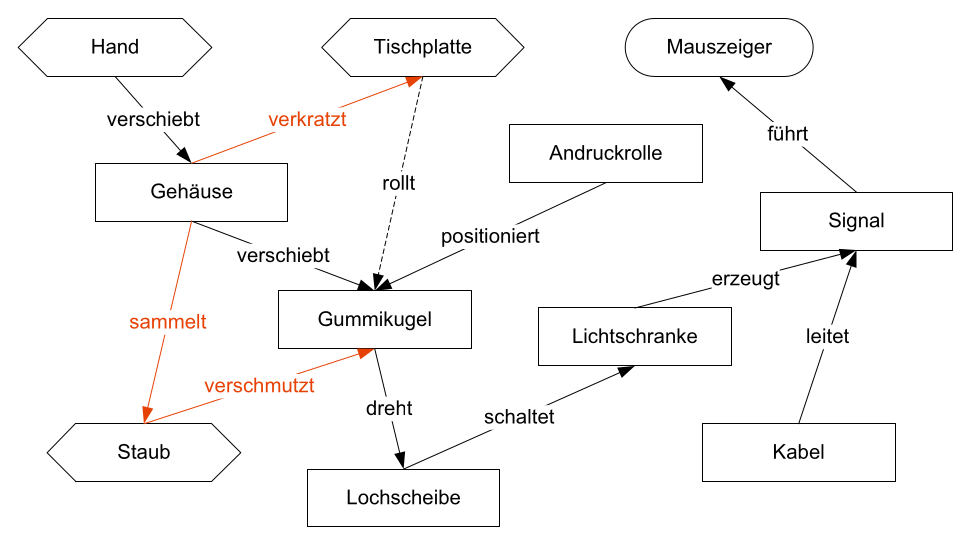
\includegraphics[scale=.6]{mouse.png}
  \caption{Functional Model For A Mechanical Computer Mouse In German}
  \label{fig:functional_model_mechanical_computer_mouse}
\end{figure}

The implementation of the function \emph{Scratches} is going to be explained.
This describes the arrow from \emph{Case (Gehäuse)} to \emph{Tabletop
  (Tischplatte)}.

The interaction is therefore \emph{CaseTabletop} with the two components
\emph{Case} and \emph{Tabletop}.  All of these are in the ex namespace as
explained in section \ref{sec:conceptualisations}.

Furthermore the action \emph{Move} is defined.  And with that the direction
\emph{CaseMoveTabletop}, by the Subject-Action-Object triple created.

Finally the quality of the function is added.  The book defined this as a
\emph{Harmful Function}.

As this is an Harmful Function an optimization is necessary.  Therefore we
define \emph{ScratchesParameter} which is a \emph{functionWithMatrixParameter}
concept.  Hence we have to choose the decreasing and increasing parameters.
As in this paper also the Matrix 2003 was implemented.  This is the one chosen
to find a suitable principle.

As an increasing parameter \emph{Power} is chosen, because the moving of the
mouse increases the working possibilities of the mouse.  The decreasing
parameter is \emph{Loss Of Material}, as the tabletop looses material during
the moving of the mouse.

With the chosen parameters the matrix entry can be obtained.  In this case
this would be \emph{$<$http://opendiscovery.org/rdf/Matrix/E.18.25$>$}.

From there the principle \emph{tc:FlexibleCoversOrThinFilms} is picked.

This should lead to an optimization for the function.  Here it could be adding
a layer between the tabletop and the mouse, like a mouse-pad.

\section{Conclusion}
\label{sec:conclusion}

This paper implemented a suggestion for an ontology for Functional Analysis.
Most of the information were taken from the book "Systematische
Innovationsmethoden" and the talk from Nikolai Shchedrin.  This gives a good
summary over all the concepts which are need for a Functional Model and the
Functional Analysis.  In a next step other sources could be added and the
ontology could be advanced.

Furthermore the examples could be made more specific, which would help for a
greater understanding on the topic.  An interesting aspect would also to see
multiple approaches on how to optimize a function with different principles.

As there is another update of the Matrix another implementation for this would
also be helpful.

In conclusion this implementation should give a good starting point for the
ontology for Functional Analysis, but could be advanced with more knowledge
and ideas from other sources.

\begin{thebibliography}{xxx}
\raggedright
\bibitem{Altshuller1979} Genrich Altshuller (1979).  Creativity as an exact
  science (in Russian). English version: Gordon and Breach, New York 1988.
\bibitem{Graebe2021} Hans-Gert Gr\"abe (2021). About the WUMM modelling
  concepts of a TRIZ ontology.
  \url{https://github.com/wumm-project/Leipzig-Seminar/blob/master/Wintersemester-2020/Seminararbeiten/Anmerkungen.pdf}.
\bibitem{KS} Karl Koltze, Valeri Souchkov (2017).  Systematische
  Innovationsmethoden (in German).  Hanser, Munich. ISBN 978-3-446-45127-8.
\bibitem{TESE2018} Alex Lyubomirsky, Simon Litvin, Sergei Ikovenko et al.
  (2018). Trends of Engineering System Evolution (TESE).  TRIZ Consulting
  Group. ISBN 9783000598463.
\bibitem{Shpakovsky2016} Nikolay Shpakovsky (2016). Tree of Technology
  Evolution. English translation of the Russian original (Forum, Moscow
  2010).\\ \url{https://wumm-project.github.io/TTS.html}
\bibitem{SKOS} SKOS -- The Simple Knowledge Organization System.
  \url{https://www.w3.org/TR/skos-reference/}.  
\bibitem{WUMM} The WUMM Project. \url{https://wumm-project.github.io/} 
\bibitem{Matrix2003} Matrix 2003:
  \url{https://triz-journal.com/wp-content/uploads/2018/04/Screen-Shot-2018-04-30-at-15.20.25.png}.
\bibitem{tabula} tabulapdf: \url{https://github.com/tabulapdf/tabula}.
\bibitem{deep_translator} Deep Translator:
  \url{https://pypi.org/project/deep-translator/}.
\bibitem{WebinarFunctionAnalysis} Nikolai Shchedrin (2020). Webinare des
  TRIZ-Ontologie-Projekts "Funktion" und "Funktionsanalyse".
\bibitem{SouchkovGlossary} Valeri Souchkov (2018). Glossary of TRIZ and
  TRIZ-related terms.
\bibitem{ShchedrinUsefulFunctionDisadvantage} Nikolai Shchedrin (2020).
  \url{https://triz-summit.ru/onto_triz/mod/metod/triz/fa/model_fa/func_syst_model/func/func_type/disadv_f/}.
\end{thebibliography}

\end{document}

